\section{La promesa de los lenguajes no nativos}

\begin{frame}[t]{Teorema fundamental de la Ingeniería del Software}
  \begin{quote}
    All problems in computer science can be solved by another level of indirection.
  \end{quote}
  \pause
  \begin{quote}
    Except the problem of too many indirection levels.
  \end{quote}
  \hfill David Wheeler (1927 -- 2004)
  \vfill
  \pause
  \begin{columns}[t]
    \begin{column}[T]{0.3\textwidth}
      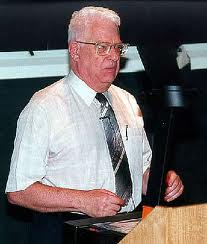
\includegraphics[width=.9\textwidth]{images/wheeler.jpg}
    \end{column}
    \begin{column}[T]{0.7\textwidth}
      \begin{itemize}
        \item Primer doctor en Informática de la historia.
        \item Inventor de la subrutina.
      \end{itemize}
    \end{column}
  \end{columns}
\end{frame}

\begin{frame}[t]{Idea fundamental}
  \begin{itemize}
    \item Write Once Run Everywhere.
      \begin{itemize}
        \item \pause Write Once \textbf{\color{red}Debug} Everywehre.
      \end{itemize}
    \item \pause El compialdor genera un código intermedio independiente del hardware que es leído y ejecutado por una máquina virtual.
    \item \pause Promesa: \textbf{\color{blue}Portabilidad}.
    \item Ejemplos:
      \begin{itemize}
        \item Java.
        \item Familia de lenguajes .NET.
      \end{itemize}
  \end{itemize}
\pause
\begin{columns}
  \begin{column}{0.2\textwidth}
    
\includegraphics[width=0.9\textwidth]{images/java.jpg}
  \end{column}
  \begin{column}{0.1\textwidth}
    
\includegraphics[width=0.9\textwidth]{images/dotnet.jpg}
  \end{column}
\end{columns}
\end{frame}

\begin{frame}[t]{Una idea novedosa}
  \begin{itemize}
    \item Idea original en \emph{O-code} de BCPL.
      \begin{itemize}
        \item Finales de los 60.
        \item Permitió portar el lenguaje BCPL a diversas máquinas.
      \end{itemize}
    \item 1966: Lenguaje BCPL.
    \item \pause 1973: \emph{p-code}
      \begin{itemize}
         \item Código de una hipotética máquina virtual.
         \item Generado en la compilación del lenguaje PASCAL.
           \begin{itemize}
             \item Compilación de PASCAL a p-code.
             \item Ejecución del p-code por una máquina virtual.
           \end{itemize}
         \item Posibilidad de construir una implementación hardware de la máquina virtual.
           \begin{itemize}
             \item 1979: PASCAL MicroEngine.
           \end{itemize}
      \end{itemize}
  \end{itemize}
\end{frame}

\begin{frame}[t]{Aspectos de p-code}
  \begin{itemize}
    \item \pause \textbf{\color{blue}Portabilidad}:
      \begin{itemize}
        \item El compilador permanece inalterado.
        \item Solamente se necesita portar el intérprete de p-code.
      \end{itemize}
    \item \pause \textbf{\color{blue}Simplicidad}:
      \begin{itemize}
        \item Se separa la generación de código independiente de la máquina de las características de un procesador concreto.
      \end{itemize}
    \item \pause \textbf{\color{blue}Tamaño}:
      \begin{itemize}
        \item El tamaño del código generado tiene a ser menor que en código máquina nativo.
      \end{itemize}
    \item \pause \textbf{\color{blue}Depuración}:
      \begin{itemize}
        \item El intérprete puede añadir comprobaciones difíciles de implementar en código nativo.
      \end{itemize}
    \item \pause \textbf{\color{blue}Rendimiento}:
      \begin{itemize}
        \item Sobrecarga que puede ser importante.
      \end{itemize}
  \end{itemize}
\end{frame}

\begin{frame}[t]{El caso de Java}
  \begin{itemize}
    \item Desarrollado en 1995 por James Gosling, Mike Sheridan y Patrick Naughton.
    \item Una instancia más de la idea de p-code:
      \begin{itemize}
        \item p-code $\rightarrow$ bytecode.
        \item p-machine $\rightarrow$ Java Virtual Machine.
        \item PASCAL MicroEngine $\rightarrow$ Java Processor (múltiples intentos).
      \end{itemize}
    \item \pause Ideales:
      \begin{enumerate}
        \item \pause Simple, orientado a objetos y familiar.
        \item \pause Robusto y seguro.
        \item \pause Neutral a la arquitectura y portable.
        \item \pause Alto rendimiento.
        \item \pause Interpretado, con hilos y dinámico.
      \end{enumerate}
  \end{itemize}
\end{frame}


\begin{frame}[t]{Un lenguaje robusto}
  \begin{itemize}
    \item Pros:
      \begin{itemize}
        \item Gestión automática de memoria $\Rightarrow$ Para evitar goteos de memoria.
        \item Ocultación de modelo de memoria $\Rightarrow$ Para evitar \emph{dangling references}
        \item Modelo de propagación de excepciones $\Rightarrow$ Para separar la detección y el tratamiento de errores.
      \end{itemize}
  \end{itemize}
  \pause
  \begin{columns}[t]
    \begin{column}[T]{0.5\textwidth}
      \begin{itemize}
        \item Efecto:
          \begin{itemize}
            \item Es difícil que un error haga detenerse un sistema completo.
          \end{itemize}
      \end{itemize}
    \end{column}
    \begin{column}[T]{0.5\textwidth}
      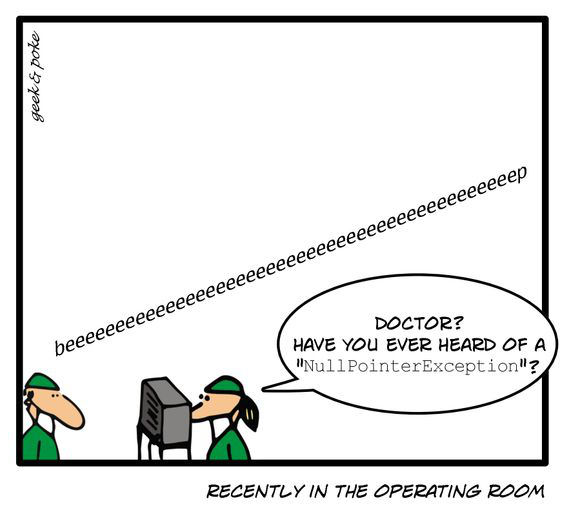
\includegraphics[height=3.5cm]{images/null-pointer-exception.png}
    \end{column}
  \end{columns}

        %\item Pero \ldots
        %  \begin{itemize}
        %    \item ¿Quién no ha visto nunca un \texttt{NullPointerException}?
        %  \end{itemize}
\end{frame}

\begin{frame}[t]{Los goteos de memoria son cosa de C++}
\begin{center}
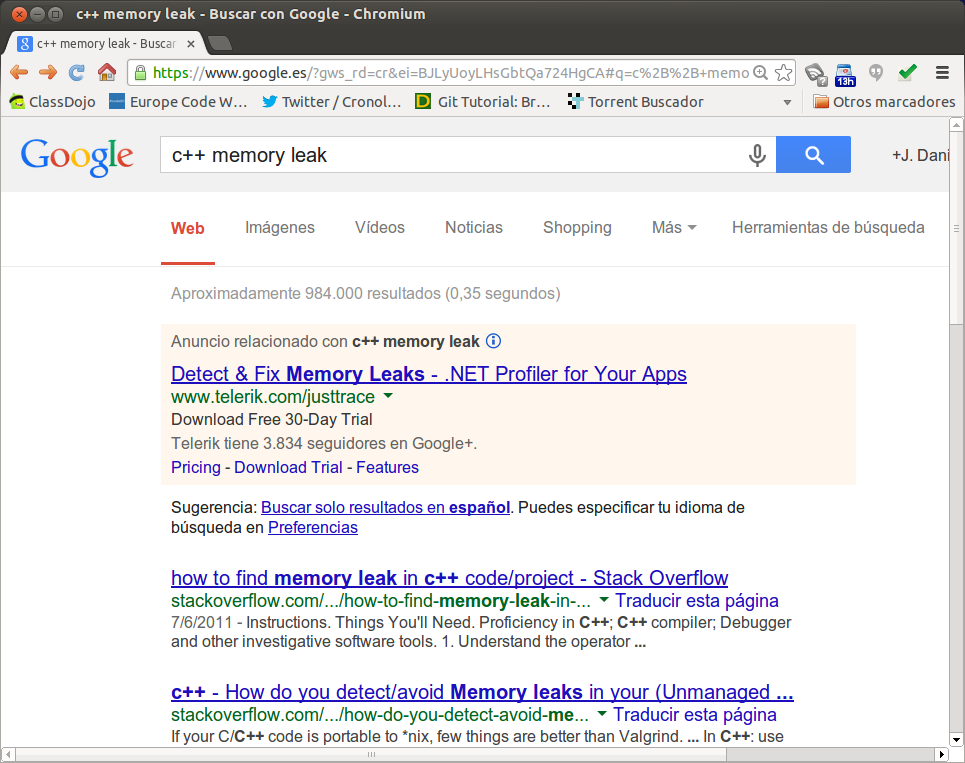
\includegraphics[width=.7\textwidth]{images/cpp-leak.png}
\end{center}
\end{frame}

\begin{frame}[t]{Java resuelve el problema}
\begin{center}
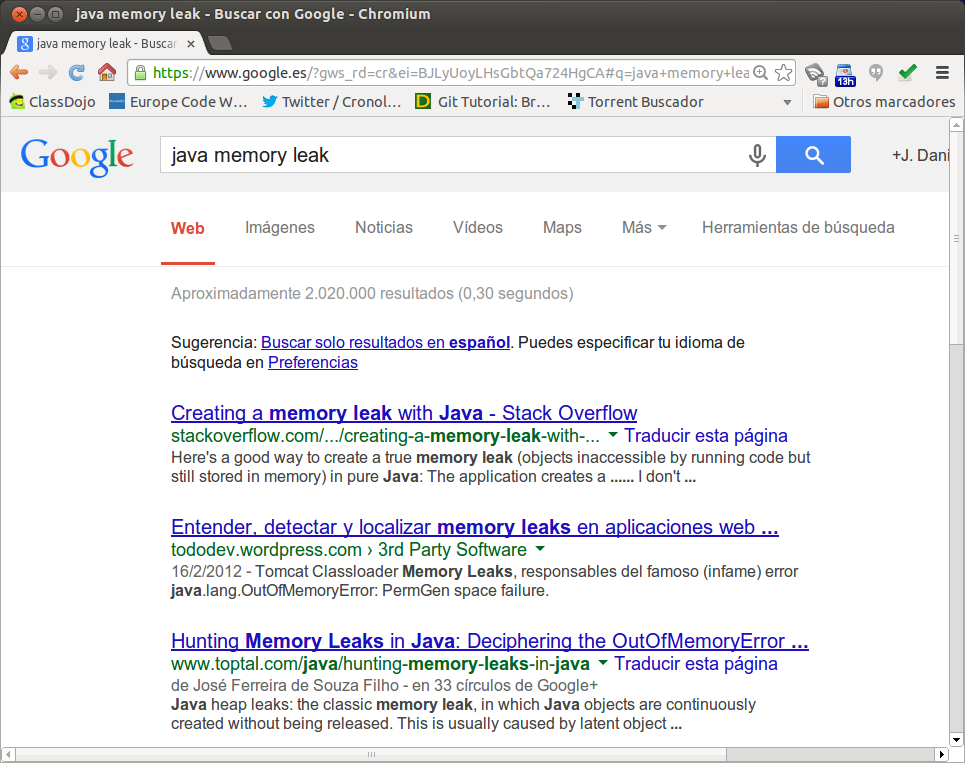
\includegraphics[width=.7\textwidth]{images/java-leak.png}
\end{center}
\end{frame}

\begin{frame}[t]{Pero por lo menos es seguro}
\begin{center}
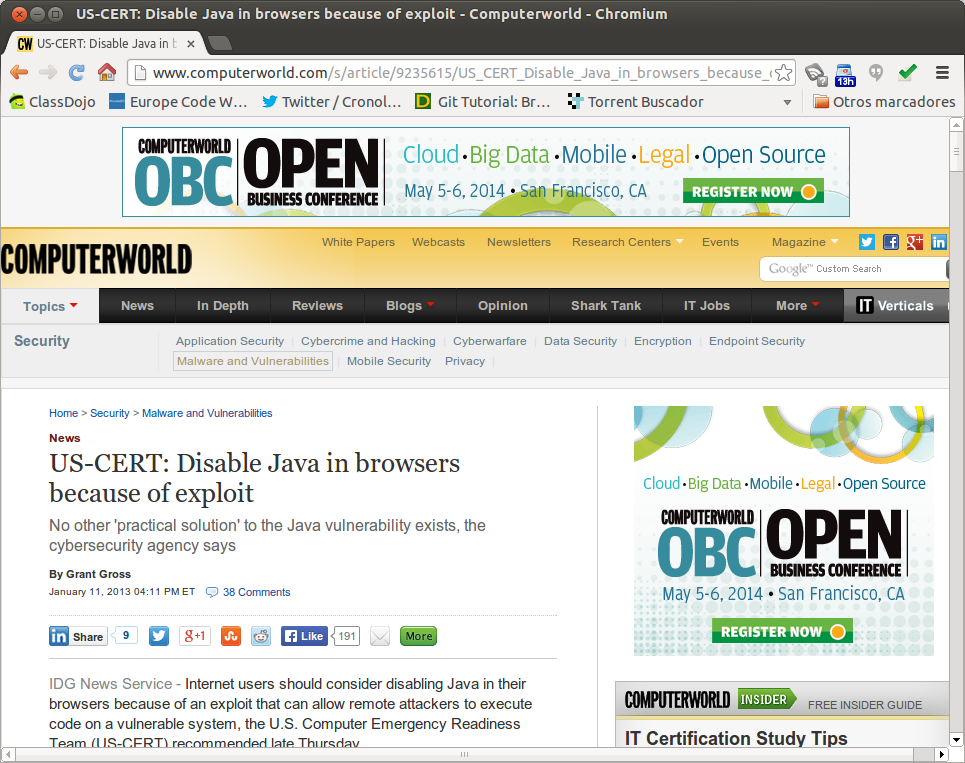
\includegraphics[width=.7\textwidth]{images/java-cert.png}
\end{center}
\end{frame}

\begin{frame}[t]{Alto rendimiento}
\begin{center}
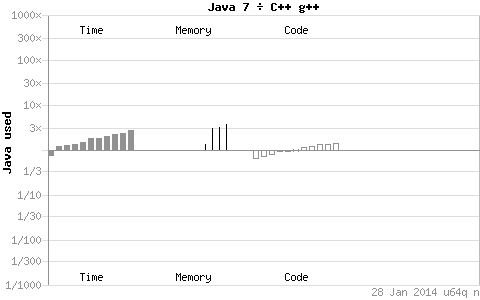
\includegraphics[width=.7\textwidth]{images/java-cpp-performance.png}

{\tiny\url{http://benchmarksgame.alioth.debian.org/u64q/benchmark.php?test=all&lang=java&id=5&data=u64q}}
\end{center}
\end{frame}
